\subsection{Effect of Memory Bandwidth Throttling}

To determine the how sensitive the model is to the shared DRAM 
memory, we use MemGuard, a memory bandwidth reservation system that 
can limit the amount of bandwidth each core receives in a period. For 
all tests run using MemGuard, we use a period of one second. 

\begin{figure}[h]
  \centering
  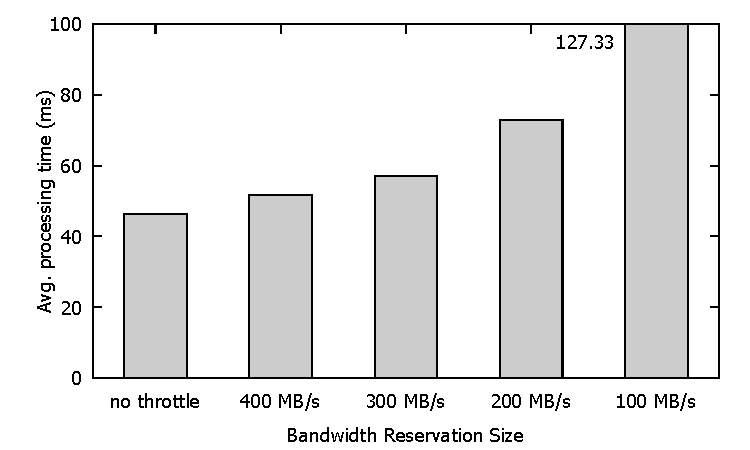
\includegraphics[width=.45\textwidth]{figs/memguard_multicore}
  \caption{Average control loop execution time vs.
    memory bandwidth reservation size. }
  \label{fig:memguard_multicore}
\end{figure}

We first run a single model on one core, Core 0, while varying the 
core's bandwidth reservation size, from 400 MB/s down to 100 MB/s. 
The results can be seen in Figure \ref{fig:memguard_multicore}. When less 
memory bandwidth is available to the core the model's performance 
noticably decreases, and it performs the best when no memory bandwidth 
throttling is implemented. Compared to a reservation size of 100 
MB/s, disabling memory bandwidth throttling results in 
\textasciitilde3x performance improvement. If the model was memory 
insensitive, then the amount of bandwidth avaiable to it would have 
little effect on its performance. However, since that is not the 
case, we conclude that, to a notable extent, the neural network model 
is dependent on shared DRAM memory performance.

\begin{figure}[h]
  \centering
  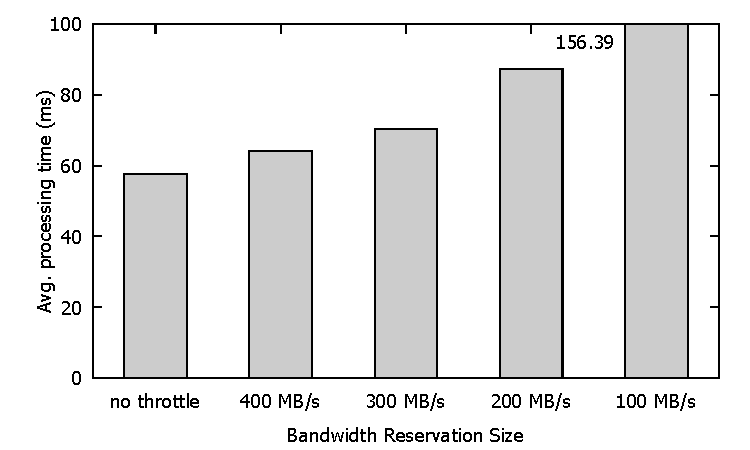
\includegraphics[width=.45\textwidth]{figs/memguard_multimodel}
  \caption{Timing impact of co-scheduling multiple DNNs when memory
bandwidth throttling is enabled. }
  \label{fig:memguard_multimodel}
\end{figure}

We also test the effects of memory bandwidth throttling in the case 
of multiple models running concurrently on the Pi 3 by rerunning the 
4Nx1C experiment. We use the same memory bandwidth reservation sizes 
from the previous experiment. The results can be seen in Figure
\ref{fig:memguard_multimodel}. Once again, the performance of the 
models are affected by the amount of memory bandwidth that is 
available to the Pi 3's cores during each period, meaning that they 
are all memory dependent.

\begin{figure}[h]
  \centering
  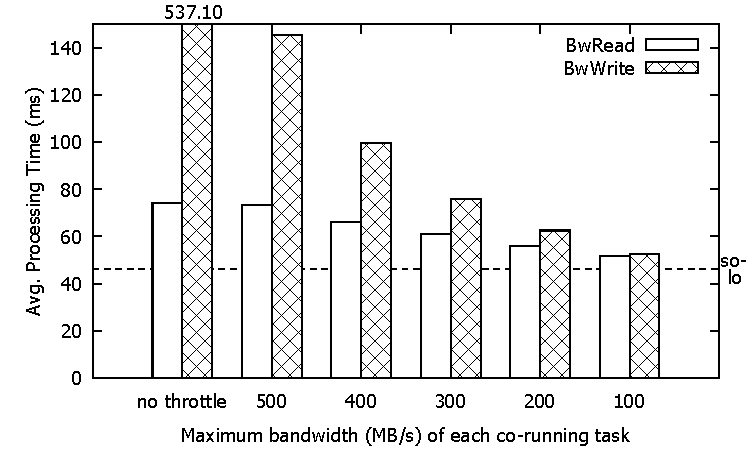
\includegraphics[width=.45\textwidth]{figs/memguard_bandwidth}
  \caption{Timing impact of co-scheduling memory intensive read
co-runners when memory bandwidth throttling is enabled. }
  \label{fig:memguard_bandwidth}
\end{figure}

Finally, we test the performance of the model in the presence of 
memory intensive read co-runners in order to determine the effects of 
limiting the memory bandwidth of the co-runners. For each of the 
experiments, we give the model's core, Core 0, a constant 1000 MB/s 
memory bandwidth reservation, and then vary the amount of bandwidth 
the co-runners' cores receive following the same scheme used in the 
previous experiments. The results can be see in Figure
\ref{fig:memguard_bandwidth}. When less memory bandwidth is given to 
the read co-runners, the performance of the model does improve. In 
the case of one co-runner, the performance of the model remains 
constant even as the reservation sizes are decreased, however, it 
still improves compared to when throttling wasn't enabled. With two 
and three co-runners, performance continually improves as less 
bandwidth is given to the benchmarks. This is especially true with 
three co-runners as the improvement is linear, which indicates that 
there is a direct correlation between the co-runner bandwidth size 
and model performance. In all cases, model performance improved, to 
some extent, through the use of memory bandwidth throttling on the 
co-runners. Since this would not be the case if the model was memory 
insensitive, we find that the model is memory dependent in the 
presence of co-runners.

Based on all of the memory bandwidth throttling experiments 
performed, it is evident that the model is dependent on the shared 
DRAM memory, to a noticable extent. When a single or multiple models 
were run, their performance(s) decreased as less memory bandwidth was 
made available to them. Furthermore, when the bandwidths of memory 
intensive read co-runners were limited, the performance of the model 
increased. As such, we conclude that the model is dependent on the 
performance of the shared DRAM memory.